%% EXERCICIOS PARA INCLUÍR DENTRO DO CADERNO DE EXERCICIOS %%
%
% EXERCICIO.- COMENTARIO AUDICIÓN PUER NATUS EST NOBIS
%
\section{Un introito gregoriano: «Puer natus est»}
%
O canto gregoriano é un dos fenómenos musicais máis importantes e identificativos da cultura 
musical occidental. Naceu coa primitiva igrexa cristiá, con influencias dos cantos de tradición 
xudea e greco-romana.
%
Dentro das propostas de análise de audición con partitura, de monodia relixiosa medieval, estudamos o «Puer natus est», un introito gregoriano.

\vspace*{0.25cm}

% Partitura de audición:
% ----------------------
\begin{figure}[h]
    \centering
    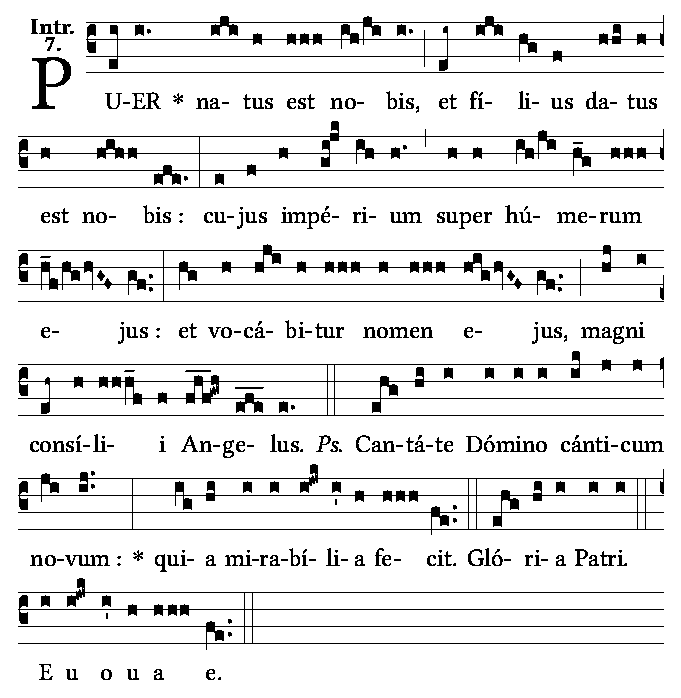
\includegraphics[width=0.60\textwidth]{figures/audicions/Puer-natus.eps}
    \caption{Partitura do Introito «Puer natus est»}
    \label{fig:puer-natus}
\end{figure}
% -----------------------
%
\subsection*{Aspectos a determinar na audición da obra}
%
%\begin{enumerate}[1.-]
%PUNTO NÚMERO 1: ESCOITAR A PEZA
%
No caso de análise dunha audición con partitura debemos prestar atención a tódolos elementos formais que observamos na partitura, como grafías e escrita (notación); son elementos que debemos recoñecer a golpe de vista. Presta moita atención á partitura e identifícaos.

Unha vez observada a partitura e os seus elementos formais, faremos unha escoita activa da obra, tratando de seguir a partitura e identificando deste xeito os elementos formais que observamos. 
%
%\begin{multicols}{2}
%
    \begin{enumerate}[1.-]
        %
        \item % RITMO
        \textbf{Ritmo}: para identificar o ritmo, debes prestar atención a aspectos como:
        pulso, relación música-texto, indicacións de compás e indicacións dinámicas, entre outras.
        \par
        Trata de identificar se estamos ante ritmo medido (mensural) ou máis ben libre (non mensural). 
        \begin{itemize}
            \item A cal dos dous se axusta? \dotfill
        \end{itemize}
        %
        \item %MELODÍA:
        \textbf{Melodía}: fixaremos a atención agora nos aspectos melódicos, para determinar o modo, ámbito e estilo. \par
        Debemos observar o perfil melódico, a interválica, se hai grandes saltos ou mais ben discorre por graos conxuntos.
%        \begin{multicols}{2}
        \begin{itemize}
            \item 
            Cal é o salto mais grande que atopas? \dotfill
            \item 
            Que intervalos se repiten con maior frecuencia? \dotfill
            \item
            Podemos afirmar que a melodía se move por graos \dotfill
        \end{itemize}
%        \end{multicols}
        Vexamos a continuación o Modo, Ámbito e Estilo:
        \begin{itemize}
            \item 
            \textbf{Modo}.- 
%        \begin{itemize}
            \begin{multicols}{2}
%            \item 
            - identifica a clave \dotfill
%            \item 
            \par
            - cal é a nota \textit{finalis}? \dotfill
%            \item
            \par
            Tendo en conta a nota final, \par
            - en que modo básico estamos? \dotfill
%            \item
            \par
            - cal é a nota máis agura? \dotfill 
            \par
            - que intervalo forma coa final? \dotfill
            \par
            - cal é a nota máis grave? \dotfill 
            \par
            - cal é a nota tenor? \dotfill 
            \par
            Tendo en conta o anterior:
            \par
            - en qué modo esta a obra? \dotfill
            \par
            \end{multicols}            
%        \end{itemize}            
            \item % PENDIENTE DE ELABORAR%
            \textbf{Ámbito}.-
            \item
            \textbf{Estilo del canto}.-
        \end{itemize}
        \begin{multicols}{2}
        \begin{itemize}
            \item 
            Son longas ou curtas? \dotfill
            \item 
            Que figuras empregan? \dotfill
            \item
            Cal é o seu ámbito? \dotfill
            \item
            Móvense por graos conxuntos ou por saltos? \dotfill
            \item
            Que perfil teñen (ascendente, descendente, en arco, etc.)? \dotfill
            \item
            Repítese a melodía? Cantas veces? \dotfill
            \item
            Que instrumentos levan as melodías principais? \dotfill
        \end{itemize}
        \end{multicols}
%
        \item % TIMBRE
        \textbf{Timbre}: identificamos os instrumentos e voces que interveñen, prestando atención en cales teñen máis relevancia. Se non coñecemos ben algún timbre podemos determinar a familia instrumental á que pertence (cordófono, aerófono, membranófono, idiófono).
        \par %Pregunta sobre o timbre
        - Que timbres recoñeces na audición? \dotfill
        \par % Consello:
        Se non recoñeces algún, podes anotar aquelas características que escoitas, para tentar identificalo posteriormente.
        %
 %
        \item %TEXTURA
        \textbf{Textura}: prestaremos atención a como se ensamblan as diferentes voces:
            \begin{enumerate}[a)]
                \item Texturas melódicas: 
                \begin{itemize}
                    \item
                    De escrita horizontal: 
                    \begin{itemize}
                        \item 
                        \textbf{textura monódica}: unha única liña melódica onde todos interpretan o mesmo
                        \item
                        \textbf{textura polifónica}: varias liñas melódicas interpretadas todas á vez   
                    \end{itemize}
                    \item
                    De escrita vertical: 
                    \begin{itemize}
                        \item 
                        \textbf{textura homofónica} ou \textbf{harmónica}: unha melodía principal acompañada por acordes
                    \end{itemize}
                \end{itemize}
                \item
                Texturas non melódicas
            \end{enumerate}
            \par %Pregunta sobre a textura
            - Que tipo de textura recoñeces na audición? \dotfill
            \par % Consello:
            Presta atención ao que escoitas e indica se so hai melodía, melodía con acompañamento, que fai o acompañamento en relación á melodía principal, (...).
%
        \item % RITMO:
        \textbf{Ritmo}: identificaremos o comportamento da rítmica dentro da peza que escoitemos.
        \begin{itemize}
            \item 
            Hai ritmo constante ou cambiante? \dotfill
            \item
            É rápido, lento, marcado, libre, (...)? \dotfill
            \item
            Identificas algún compás (división, subdivisión, (...)? \dotfill
            \item
            Escoitas algunha voz leva o ritmo? Cal? \dotfill
        \end{itemize}
%
        \item % HARMONÍA:
        \textbf{Harmonía}: identificaremos, no caso de texturas homofónicas, tonalidade, modalidade, atonalidade. No caso de pezas polifonía, hai que fixarse tamén no uso de consonancias ou disonancias.
        \par %Pregunta sobre a textura
        - Segundo a textura da peza, podemos dicir que hai algún tipo de acompañamento harmónico? \dotfill
%
        \item %FORMA:
        \textbf{Forma}: despois de escoitar a peza completa, farémonos unha idea dos instrumentos, da extensión (duración) que ten e tamén da estrutura. Debemos identificar aquí, se é o caso, cales son as partes (seccións, movementos, ...) da obra ou peza e que trazos ten cada unha delas. Dentro dos tipos de formas que debemos coñecer, identificaremos:
            \begin{enumerate}[a)]
                \item
                Segundo a extensión:
                \begin{itemize}
                    \item
                    \textbf{Formas maiores}, de diferentes movementos ou grandes dimensións
                    \item
                    \textbf{Formas menores}, un só movemento ou de curta duración
                \end{itemize}
                \item
                Segundo os instrumentos ou voces:
                 \begin{itemize}
                    \item
                    \textbf{Formas vocais}, con intervención da voz humana
                    \item
                    \textbf{Formas instrumentais}, só instrumentos
                \end{itemize}
                \item 
                Segundo a súa estrutura:
                \begin{itemize}
                    \item 
                    \textbf{Formas estruturadas}, ou fixas: aquelas con esquema compositivo determinado, como por exemplo sonatas, sinfonías, etc.
                    \item
                    \textbf{Formas libres}: non respetan aparentemente ningunha estrutura definida
                \end{itemize}
            \end{enumerate}
        \par %Pregunta sobre as Formas
        - A que tipo de forma, podemos dicir que se axusta a peza? \dotfill
        \par % Consello:
        Ten en conta, que ata o momento estamos a escoitar pequenas pezas onde se combina a voz con certos instrumentos e malia que pode semellar que non teñen un esquema compositivo fixo, pode dar lugar a confusión.    
        \end{enumerate}
%    \end{multicols}
%
\subsubsection*{Notas sobre a audición}
Redacta un breve comentario sobre a audicióno que acabamos de escoitar tendo en conta os puntos anteriores.
%
\begin{ejercicio}[Comentario resumo do \textit{Epitafio de Seikilos}]
% ESPACIO PARA REDACTAR O COMENTARIO DA AUDICIÓN
        \vspace*{2.78cm}
\end{ejercicio}
%
% --------------------------
% EXPLICACIÓN DAS AUDICIÓNS:
% --------------------------
%
%\newpage
%
%\subsection*{Recoñecemento auditivo de formas vocais e instrumentais}
%
%Escoita con atención as dúas obras que se propoñen como exercicios de audición e completa as fichas correspondentes. Procura información sobre as mesmas e sobre o autor para coñecer o seu contexto.
%\par
%\begin{multicols}{2}
%
% AUDICIÓN 3.- HIMNO A NÉMESIS
% ----------------------------
% Suite "Música acuática" de George Friedrich Haendel (1685-1759)
%
%\begin{ejercicio}[]
%
%Completa a ficha da obra proposta como exercicio de audición.
%
%	\begin{enumerate}[1.-]
%        \vspace*{0.3cm}
%		\item
%			Autor: \dotfill
%			\vspace*{0.3cm}
%		\item
%			Obra:
%			\begin{enumerate}[a)]
%			    \item Título: \dotfill \vspace*{0.3cm}
%			    \item Forma: \dotfill \vspace*{0.3cm}
%			    \item Xénero: \dotfill \vspace*{0.3cm}
%			    \item Estilo: \dotfill \vspace*{0.3cm}
%			    \item Instrumentación: \dotfill 
%			    \vspace*{0.3cm}
%			\end{enumerate}
%		\item 
%		    Resume as principais características que definen a obra:
%			\vspace*{10.0cm}			
%
%	\end{enumerate}
%\end{ejercicio}
%
% AUDICIÓN 4.- EPITAFIO SEIKILOS
% --------------------------------------------
% Oratorio "El Mesías" de George Friedrich Haendel (1685-1759)
%
%\begin{ejercicio}[]
%
%Completa a ficha da obra proposta como exercicio de audición.
%
%	\begin{enumerate}[1.-]
%        \vspace*{0.3cm}
%		\item
%			Autor: \dotfill
%			\vspace*{0.3cm}
%		\item
%			Obra:
%			\begin{enumerate}[a)]
%			    \item Título: \dotfill \vspace*{0.3cm}
%			    \item Forma: \dotfill \vspace*{0.3cm}
%			    \item Xénero: \dotfill \vspace*{0.3cm}
%			    \item Estilo: \dotfill \vspace*{0.3cm}
%			    \item Instrumentación: \dotfill 
%			    \vspace*{0.3cm}
%			\end{enumerate}
%		\item 
%		    Resume as principais características da obra:
%			\vspace*{10.0cm}			
%
%	\end{enumerate}
%\end{ejercicio}
%
%\end{multicols}
%
%\newpage
%
%
%\begin{multicols}{2}
%
% AUDICIÓN 3.- HIMNO A NÉMESIS
% ----------------------------
% Suite "Música acuática" de George Friedrich Haendel (1685-1759)
%
%\begin{ejercicio}[]
%
%Completa a ficha da obra proposta como exercicio de audición.
%
%	\begin{enumerate}[1.-]
%        \vspace*{0.3cm}
%		\item
%			Autor: \dotfill
%			\vspace*{0.3cm}
%		\item
%			Obra:
%			\begin{enumerate}[a)]
%			    \item Título: \dotfill \vspace*{0.3cm}
%			    \item Forma: \dotfill \vspace*{0.3cm}
%			    \item Xénero: \dotfill \vspace*{0.3cm}
%			    \item Estilo: \dotfill \vspace*{0.3cm}
%			    \item Instrumentación: \dotfill 
%			    \vspace*{0.3cm}
%			\end{enumerate}
%		\item 
%		    Resume as principais características que definen a obra:
%			\vspace*{13.0cm}			
%
%	\end{enumerate}
%\end{ejercicio}
%
% AUDICIÓN 4.- EPITAFIO SEIKILOS
% --------------------------------------------
% Oratorio "El Mesías" de George Friedrich Haendel (1685-1759)
%
%\begin{ejercicio}[]
%
%Completa a ficha da obra proposta como exercicio de audición.
%
%	\begin{enumerate}[1.-]
%        \vspace*{0.3cm}
%		\item
%			Autor: \dotfill
%			\vspace*{0.3cm}
%		\item
%			Obra:
%			\begin{enumerate}[a)]
%			    \item Título: \dotfill \vspace*{0.3cm}
%			    \item Forma: \dotfill \vspace*{0.3cm}
%			    \item Xénero: \dotfill \vspace*{0.3cm}
%			    \item Estilo: \dotfill \vspace*{0.3cm}
%			    \item Instrumentación: \dotfill 
%			    \vspace*{0.3cm}
%			\end{enumerate}
%		\item 
%		    Resume as principais características da obra:
%			\vspace*{13.0cm}			
%
%	\end{enumerate}
%\end{ejercicio}
%
%\end{multicols}
%